\articlehead{Carroll Ballard's Never Cry Wolf}{JM}{2013}

This is my final article looking at the great animal films of Carroll Ballard. The other articles are on \textit{The Black Stallion} (1979), \textit{Fly Away Home} (1996) before, and \textit{Duma} (2005).

It opened the way to an old—and very naïve—childhood fantasy of mine: to go off into the wilderness, and test myself against all the dangerous things lurking there. And to find that basic animal that I secretly hoped was hidden somewhere inside myself. I imagined, at that point, I’d become a new man, with a strength and courage I’d never known before.

Tyler is a nerdy biologist who has accepted an unusual task: spend 6 months, alone, in the Canadian arctic to observe the behaviour of local wolves. \textit{Never Cry Wolf} follows Tyler from spring’s thaw to the first snowfalls of the coming winter. It’s a curious film: subtle, slow, and moving. It is also a masterpiece.

\begin{figure}
  \begin{center}
    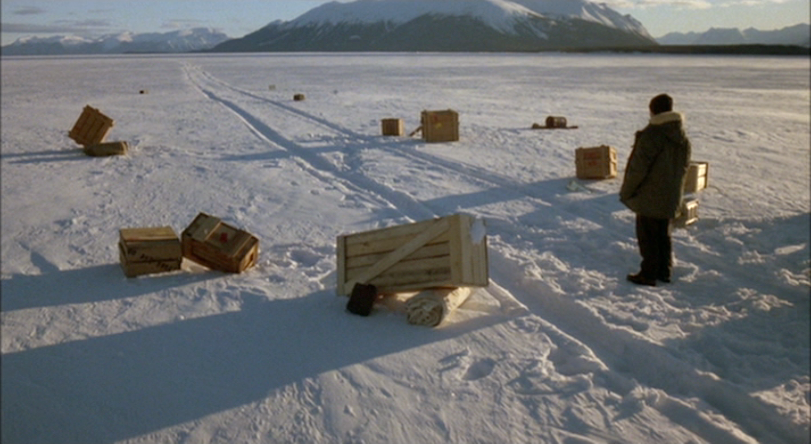
\includegraphics[width=\textwidth]{content/assets/never-cry-wolf--tyler}
  \end{center}
  \caption{Day 1 of Tyler's journey}
\end{figure}

The story is of Tyler’s relationship with wolves. Over the course of six months, he starts as a detached scientific observer, and learns to embrace his inner wolf as time goes on. (The quote at the beginning of this article is from Tyler’s voiceover narration in the first few seconds of \textit{Never Cry Wolf}.) This film is about the furry condition.

\textit{Never Cry Wolf} was filmed and released in the early 1980s, years before furry coalesced into a discrete group. In the early days of furry, it was largely a cartoon animal fandom, based around pre-existing works of art such as Disney’s Robin Hood. Nowadays, furry still has plenty of fandom elements but is more about personal identity: we choose to think of ourselves as animal-people, and we spend time in a virtual world filled with our fellow animal-people.

Tyler is an animal person: he is, essentially, a wolf furry. Over the course of the film, he learns to think of himself as an instinctual animal, rather than a purely logical being. He even has an (imaginary) wolf physical form.

Tyler is expressing a personal connection with the animal world. He is exploring something that has been a part of human spirituality for at least dozens of millennia. We furries are merely the newest manifestation of this spiritual thread.

Tyler’s furriness starts to blossom when he is introduced to some concepts of Inuit totemism. Tyler doesn’t co-opt Inuit beliefs or tradition, rather he uses some ideas as a template to create his own, personal relationship with his inner wolf. He remains a scientist and a skeptic, but slowly sheds the protective baggage he carries with himself. (Metaphor alert: some of his baggage is actual, uh, baggage, and he even hides in his baggage from some wolves early on.)

Tyler begins his personal journey after being dumped, alone, in the wilderness along with supplies for his study. The Canadian arctic in early spring is harsh and deadly. In all of Carroll Ballard’s films, there is a sense of malevolence about the natural environment: the deserted island of \textit{The Black Stallion}, the flight in flimsy ultralights in \textit{Fly Away Home}, the South African wilderness in \textit{Duma}. And so it is in \textit{Never Cry Wolf}; faced with the likelihood of exposure in freezing temperatures, Tyler makes a series of bad decisions: he defrosts a beer, types out an angry letter (in triplicate) to his superiors, and rides out his first night huddled in an upturned canoe. It’s hard to tell if he is ignorant of death’s approach, or resigned to his fate.

Tyler is eventually bundled into shelter and temporary safety by a passing Inuit. Here he dreams of being devoured by wolves, a moment that signifies the birth of his inner animal. The dream is terrifying on first viewing, but over the length of the film it takes on a mythical quality as Tyler, wolf-person, grows.

Soon after Tyler awakens, we see the first evidence that he has changed. He falls through thin ice, and saves himself through a combination of intelligence and instinct. He dries himself, and his clothes, by a fire, and we can sense that his internal journey has begun. This scene is a key turning point in the film as well.

For starters, this is the first time we see Tyler naked. It’s initially played for tittilative laughs (as in: tee hee I can see his bum), but the scene stretches until his nudity is a comfortable, natural, default state. Tyler is shedding more of his uptight human baggage, and he starts to relax, to feel at home in the wilderness.

From this moment on the film becomes hazy, soft, and beautiful; Ballard’s direction encourages the viewer to share Tyler’s surrender to the natural world. This stands in obvious juxtaposition to the tone of the preceding part of the film which is rushed, full of unconvincing danger, and a bit hammy. It’s clear that Ballard wanted to spend as little time on the preamble as possible.

Soon, Tyler comes across a wolf pack and he starts his study. He tries to hide his presence from the wolves, and fails miserably against the wolf’s senses. He quickly abandons any attempt of subterfuge, and eventually negotiates a wolf-approved territory within observing distance.

His time observing the wolves is the heart of the film. There is little action and Tyler is alone for much of the time, save for a developing friendship with two Inuit. There are two parallel stories: Tyler’s growing relationship with the wolves, and Tyler’s growing relationship with his personal, inner wolf.

This long section of the film is, to put it mildly, remarkable. Respect grows between Tyler and the wolves, to the point that they are eventually able to vocally express their fellowship, the howling of the wolves mirrored in Tyler’s bassoon. And Tyler’s inner wolf becomes more real, gaining a physical form and a personality: strong, quiet, intelligent, and protective.

The film’s high point takes place on a hazy late-summer afternoon. Tyler has reached a peace with himself and with his environment by this point, and is dozing in the sun when a herd of caribou thunder past. He becomes wondrously lost in the stampede, as the wolves gather to corral the more vulnerable members of the caribou. It’s wordless, visceral, and complex.

The flow of \textit{Never Cry Wolf} is that of the seasons. Tyler is vulnerable and naïve in the spring; learns and grows through the summer, before the contentment of autumn. His internal journey is reflected in the changing landscape and in the growth of the wolves’ family (no Ballard film would be complete without the odd cute baby animal scene). He starts as an observer and ends as a participant; his trimmed moustache grows into full beard; he begins with bureaucracy and ends in ecstatic nudity.

From a furry perspective, \textit{Never Cry Wolf} is something very special. If you feel or imagine a connection with your furry species, especially if you’re a wolf, you should take the time to track down this film. (That advice does not include anyone who identifies as a mouse. It does not go well for mice in \textit{Never Cry Wolf}.)

But even for non-furs, \textit{Never Cry Wolf} is a great film. It’s the antidote to patronizing bullshit like \textit{Dances With Wolves} or doco-lite snoozefests like \textit{March Of The Penguins}. It’s thoughtful without being moralizing, complex without being complicated, and moving without being melodramatic. As the late Roger Ebert put it, \textit{Never Cry Wolf} is a classic.

Final notes:
\begin{itemize}
  \item There is a lot of male nudity and alcohol consumption in \textit{Never Cry Wolf}. It’s unthinkable that such a film would get a PG rating in America today.
  \item Charles Martin Smith, who plays Tyler, went on to direct Air Bud, which is a live-action film about a dog that plays basketball. From the sublime to the ridiculous.
\end{itemize}

\textit{Never Cry Wolf} is available on iTunes.

This is the final of four articles on the films of Carroll Ballard. All four films are great. Choose your species:

\begin{itemize}
  \item \textit{The Black Stallion} (horse)
  \item \textit{Never Cry Wolf} (wolf)
  \item \textit{Fly Away Home} (goose)
  \item \textit{Duma} (cheetah)
\end{itemize}
